\subsection{Pracovní postup}
    Nejprve bylo potřeba očistit keramický substrát od starých součástek a zbytků pájecí slitiny. Následně mohla být dispenzerem nanesena pájecí pasta a do ní za pomocí vakuové pipety usazeny nové rezistory. K této úloze byla použita pájecí slitina SAC 305. Na základě ověřeného pájecího profilu (viz \ref{profilek}) jsme osazený substrát podrobili procesu pájení přetavením ve stejné pájecí peci. Následně jsme za pomoci optického mikroskopu zhodnotili kvalitu pájených spojů, ukázka je vidět na Obr. \ref{fig:img-kvalita-jpg}.

    \begin{figure}[h!]
        \centering
        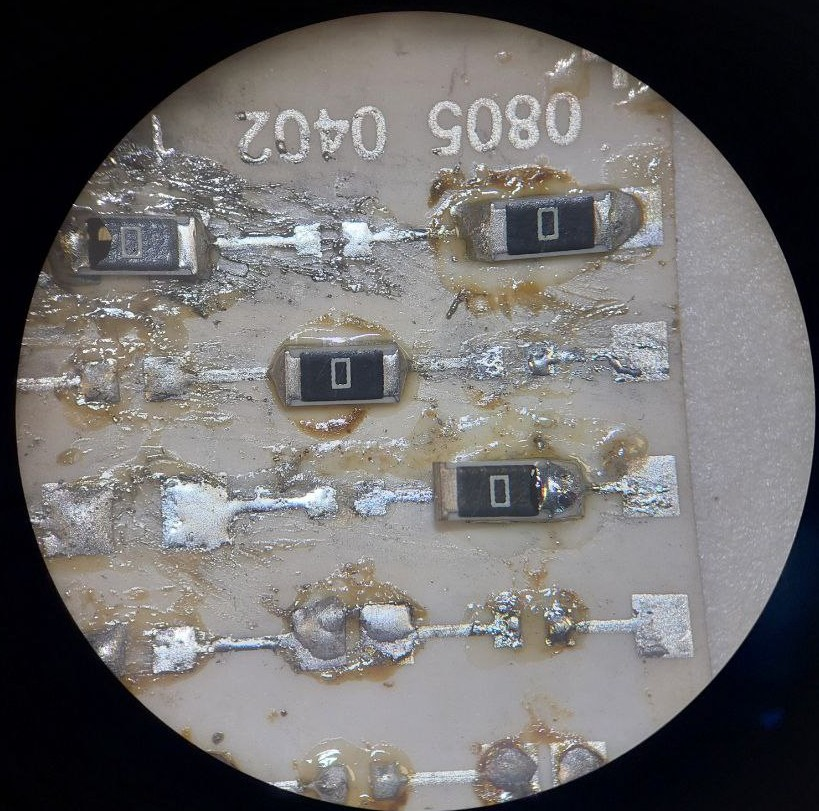
\includegraphics[width=0.6\textwidth]{img/kvalita.jpg}
        \caption{Posouzení kvality pájeného spoje.}
        \label{fig:img-kvalita-jpg}
    \end{figure}
    

\subsection{Leaching}
    U tří různých pájecích past jsme testovali možnost vzniku leachingu při pájení přetavením. K testu byl použit keramický substrát na kterém je vodivý motiv vytvořen tiskem tlustovrstvé stříbrné pasty. Na stejný substrát byl umísten vzorek každé z pájecích past, onkrétně se jednalo o pasty Sn63Pb37, Sn42Bi58 a SAC305. K dosažení leatchingu jsme si pomohli vyšší teplotou, než je optimální pro tyto pasty, tedy cca \qty{250}{\degreeCelsius}. Výsledek našeho pozorování je vidět na Obr. \ref{fig:img-leatching-jpg}

    \begin{figure}[h!]
        \centering
        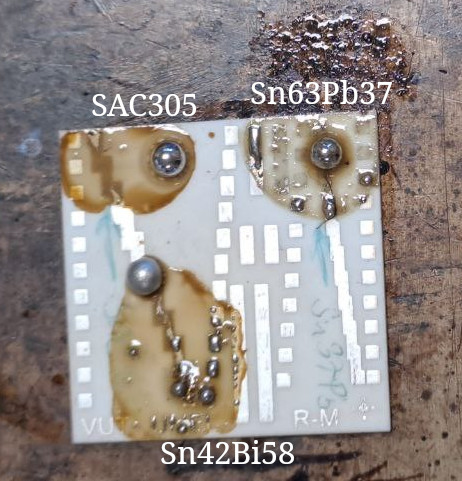
\includegraphics[width=0.6\textwidth]{img/leatching.jpg}
        \caption{Ukázka jevu leatching pro různé pájecí pasty.}
        \label{fig:img-leatching-jpg}
    \end{figure}
    



\subsection{Měření teplotního profilu} \label{profilek}
    U konvekční přetavovací pece (Essemtec RO 300FC) jsme testovali nastavení pájcího profilu. Zkouška probíhala za pomocí testovacího substrátu osazeného termočlánky připojenými k měřícímu přípravku. Změřený pájecí profil se nachází na Obr. \ref{graf:profil}, můžeme na něm vidět průbeh měřené teploty z obou termočlánků a také ze sensorů zabudovaných napevno v jednotlivých zónách pece, které by měly reflektovat nastavené teploty.

    \begin{figure*}[h!]
        \begin{tikzpicture}
            \centering
            \begin{axis}
                [
                xlabel={\( t\ [\unit{\second}]\)},
                ylabel={\( T\ [\unit{\degreeCelsius}]\)},
                %axis y line*=left, % dve y osy
                width=1\textwidth,
                height = 0.5\textwidth,
                legend pos=north west
    %			xmin=0,
    %			ymin=0,
    %			xmax=100
    %			ymax=100
                ]
    
                \addplot[mark=none, mark options={solid}, thick,  red, solid, mark size=3pt] table [skip first n=0, x=Zone-1-X, y=Zone-1-Y, col sep=comma] {data/profil.csv};
                \addlegendentry{Zone-1-}
    
                \addplot[mark=none, mark options={solid}, thick,  green, solid, mark size=3pt] table [skip first n=0, x=Zone-2-X, y=Zone-2-Y, col sep=comma] {data/profil.csv};
                \addlegendentry{Zone-2-}
    
                \addplot[mark=none, mark options={solid}, thick,  yellow, solid, mark size=3pt] table [skip first n=0, x=Zone-3-X, y=Zone-3-Y, col sep=comma] {data/profil.csv};
                \addlegendentry{Zone-3-}
    
                \addplot[mark=none, mark options={solid}, thick,  black, solid, mark size=3pt] table [skip first n=0, x=Sonda-1-X, y=Sonda-1-Y, col sep=comma] {data/profil.csv};
                \addlegendentry{Sonda-1-}
    
                \addplot[mark=none, mark options={solid}, thick,  gray, solid, mark size=3pt] table [skip first n=0, x=Sonda-2-X, y=Sonda-2-Y, col sep=comma] {data/profil.csv};
                \addlegendentry{Sonda-2-}
                
            \end{axis}   
        
            
        \end{tikzpicture}
        \caption{Měřený teplotní profil.}
        \label{graf:profil}
    \end{figure*}